\documentclass[12pt,a4paper]{article}
\usepackage[utf8]{inputenc}
\usepackage[T1]{fontenc}
\usepackage{amsmath}
\usepackage{amsfonts}
%\usepackage{amssymb}
\usepackage{bbm}
\usepackage{graphicx}
\usepackage{geometry}
\usepackage{enumitem}
\usepackage{hyperref}

\usepackage{exsheets}
\SetupExSheets{counter-format=ch.qu}

\geometry{a4paper, margin=2cm}

\usepackage{cprotect}

\usepackage{xcolor}
\definecolor{maroon}{cmyk}{0, 0.87, 0.68, 0.32}
\definecolor{halfgray}{gray}{0.55}
\definecolor{ipython-frame}{RGB}{207, 207, 207}
\definecolor{ipython-bg}{RGB}{247, 247, 247}
\definecolor{ipython-red}{RGB}{186, 33, 33}
\definecolor{ipython-green}{RGB}{0, 128, 0}
\definecolor{ipython-cyan}{RGB}{64, 128, 128}
\definecolor{ipython-purple}{RGB}{170, 34, 255}

\usepackage{listings}
\lstdefinelanguage{iPython}{
	morekeywords={access,and,del,except,exec,in,is,lambda,not,or,raise},
	morekeywords=[2]{for,print,abs,all,any,basestring,bin,bool,bytearray,callable,chr,classmethod,cmp,compile,complex,delattr,dict,dir,divmod,enumerate,eval,execfile,file,filter,float,format,frozenset,getattr,globals,hasattr,hash,help,hex,id,input,int,isinstance,issubclass,iter,len,list,locals,long,map,max,memoryview,min,next,object,oct,open,ord,pow,property,range,reduce,reload,repr,reversed,round,set,setattr,slice,sorted,staticmethod,str,sum,super,tuple,type,unichr,unicode,vars,xrange,zip,apply,buffer,coerce,intern,elif,else,if,continue,break,while,class,def,return,try,except,import,finally,try,except,from,global,pass, True, False},
	sensitive=true,
	morecomment=[l]\#,%
	morestring=[b]',%
	morestring=[b]",%
	moredelim=**[is][\color{black}]{@@}{@@},
	identifierstyle=\color{black}\footnotesize\ttfamily,
	commentstyle=\color{ipython-cyan}\footnotesize\itshape\ttfamily,
	stringstyle=\color{ipython-red}\footnotesize\ttfamily,
	keepspaces=true,
	showspaces=false,
	showstringspaces=false,
	rulecolor=\color{ipython-frame},
	frame=single,
	frameround={t}{t}{t}{t},
	backgroundcolor=\color{ipython-bg},
	basicstyle=\footnotesize\ttfamily,
	keywordstyle=[2]\color{ipython-green}\bfseries\footnotesize\ttfamily, 
	keywordstyle=\color{ipython-purple}\bfseries\footnotesize\ttfamily
}

\lstdefinelanguage{iOutput} {
	sensitive=true,
	identifierstyle=\color{black}\small\ttfamily,
	stringstyle=\color{ipython-red}\small\ttfamily,
	keepspaces=true,
	showspaces=false,
	showstringspaces=false,
	rulecolor=\color{ipython-frame},
	basicstyle=\small\ttfamily,
}

\lstnewenvironment{ipython}[1][]{\lstset{language=iPython,mathescape=true,escapeinside={*@}{@*}}%
}{%
}

\lstnewenvironment{ioutput}[1][]{\lstset{language=iOutput,mathescape=true,escapeinside={*@}{@*}}%
}{%
}

\title{Addons with Python Exercises}
\author{Matteo Sani}

\begin{document}
\maketitle

\section{Stochastic Simulation}
In science, we are often more interested in the distribution of a set of outcomes rather than a single event. This may be the probability distribution of a molecule diffusing a specific distance as a function of time, or the price change of a very exotic derivative.

Stochastic simulations allow us to generate a series of experiments on a system in which one step is governed by random chance. These simulations often boil down to flipping a coin to dictate if said step will occur or not.

Of course, sitting in your office chair flipping a coin over and over again is not how one should do a simulation. To get a sense of the probability distribution of some outcome, we often have to simulate the process thousands of times. This means that we need to know how to make our computers do the heavy lifting.

It's often easy to forget just how powerful modern computers can be. What once required a serious computational cluster only twenty years ago can now be done on a 10 mm thick compartment made of rose-gold colored aluminium. 

%FIXME few words about mean and C.L.

\subsection{1D Random Walk}
The Random Walk in one dimension is a model for each process which have simple binary outcomes.

The 1D random walk can be used to model how a gambler plays a game such as roulette in a casino. The idea in such games is that the gambler places a small stake on each game (say 1€). When the game is played the gambler will either loose and the total amount of money he has will thus decrease by one unit, or alternatively, he will win the game and in that case he wins back his stake and a prize, which we will set as 1€. As you can see if the gambler repeats this process of staking money and playing the amount of money he has will undergo a random walk in one dimension, since the outcome will be either 1 or -1.

\begin{question}
Code a function that simulate a 1D random walk. 

\noindent
\textbf{Hint:} we can decide whether to walk left or right by flipping a coin and seeing if it comes up \emph{heads} or \emph{tails}.
\end{question}

\subsubsection{Simulating a Gambler}

Importantly there is a difference between the gambler and the 1D random walk, however. The gambler usually only has a finite amount of money to gamble with. If he looses a large number of games he is therefore forced to stop playing. Similarly, the gambler may also have some target for how much money he would like to win. In other words, he should have some figure $N$€, which is more than the amount of money he entered the casino with. He will stop gambling once he has $N$€ in his pocket.

\begin{question}
Determine with a simulation the probabilities whether the gambler leaves the casino with zero or with $N$€.

Essentially we start the gambler with $X$€ and simulate the process of him playing the game only stopping once he has reached one of the two thresholds.

Write a function called gambler that simulates this procedure, taking three arguments:
\begin{itemize}
\item \texttt{start}: the amount of money the gambler starts with; \item \texttt{n}: the target amount of money that the gambler wants to win;
\item \texttt{p}: the probability of winning each individual game the gambler plays.
\end{itemize}
\end{question}

We can also use simulation to determine how many spins of the wheel the gambler will play before leaving the casino (i.e. \emph{hitting time}).
In other words we want to calculate the number of steps the random walk takes before arriving in one of the two threshold states.

\begin{question}
Write another function that simulates the changes in the amount of money the gambler has and that returns the number of spins of the wheel that take place.
\end{question}

\section{Martingale Examples}
Suppose you play the following series of games. In game $i, i = 1, 2,\ldots$, you bet \$1 and roll a fair die. If the outcome is $\{1,2\}$ you win \$1, if it is $\{3,4\}$ nothing happens, and if the outcome is $\{5,6\}$ you lose \$1.
Let $X_i$ be a random variable representing the amount of money you win or lose in bet $i$, this kind of game is said to be **fair** since

$$\mathbb{E}[X_i]= \sum_{\Omega}p(\omega)\cdot x(\omega) = \frac{2}{6}\cdot 1 + \frac{2}{6}\cdot 0 + \frac{2}{6}\cdot -1 = 0\;\forall i$$
so no unbalance between losses or wins.

Now define another random variable $Z_n = \sum_{i=1}^{n} X_i$, i.e. the amount of money held at the $n$-th game.

$Z_n$ is a martingale and $\mathbb{E}[Z_n|X_1,\ldots, X_{n-1}] = Z_{n-1}$.

\paragraph{Proof}

\begin{equation}
	\begin{aligned}
		\mathbb{E}[Z_n|X_1,\ldots, X_{n-1}] &= \mathbb{E}[X_1 +\ldots + X_n|X_1,\ldots, X_{n-1}] \\
		& = \underbrace{\mathbb{E}[X_1|X_1,\ldots, X_{n-1}]}_{X_1} + \ldots + \underbrace{\mathbb{E}[X_{n-1}|X_1,\ldots, X_{n-1}]}_{X_{n-1}} + \underbrace{\mathbb{E}[X_n|X_1,\ldots, X_{n-1}]}_{\mathbb{E}[X_n]=0} \\
		& = \mathbb{E}[X_1|X_1,\ldots, X_{n-1}] + \ldots + \mathbb{E}[X_{n-1}|X_1,\ldots, X_{n-1}] + 0 = Z_{n-1}
	\end{aligned}
\end{equation}

\begin{question}
Using Monte Carlo simulation implement the game described in the text and check that the expected gain is indeed null.
\end{question}

\begin{question}
An unbiased random walk (in any number of dimensions) is another example of a martingale.

In higher dimensions, the set of randomly walked points has interesting geometric properties. In fact, one gets a discrete \emph{fractal}, that is, a set that exhibits stochastic self-similarity on large scales.

Implement a 2D random walk simulation and plot one possible realization.
\end{question}

\section{Simulating Stochastic Differential Equations}

Consider a generic stochastic differential equation (SDE)

\begin{equation}
dX(t) = \mu(t,X(t))dt + \sigma(t,X(t))dW(t)
\label{eq:sde}
\end{equation}

The Monte Carlo simulation of such a process can be carried out according to the \emph{Euler scheme} as follows: conisider the value of $X$ at time $t=t_i$, the value compute $X(t_{i+1})$ is evaluated from the dynamics of X (Eq.\ref{eq:sde}), setting $\Delta t = t_{i+1} - t_{i}$, and sampling from a standard normal $\mathcal{N}(0,1)$ in order to "evolve" the stochastic term $dW$
\begin{equation}
X(t_{i+1}) = X(t_i) + \mu(t_i,X(t_i))\Delta t + \sigma(t_i,X(t_i))\sqrt{\Delta t}\mathcal{N}(0,1)
\end{equation}

In the specific case of a simple brownian motion the dynamics is given by
\begin{equation}
dW = \sqrt{dt}\mathcal{N}(0,1)
\end{equation}
so
\begin{equation}
W(t+dt) = W(t) + \sqrt{dt}\mathcal{N}(0,1)
\end{equation}
or
\begin{equation}
W(t) = \sum_{t_0}^{t} \sqrt{dt}\mathcal{N}(0,1)
\end{equation}

Figure|\ref{fig:brownian_motion} reports two realization of the Brownian motion simulated according to the Euler scheme.

\begin{figure}[htbp]
\begin{center}
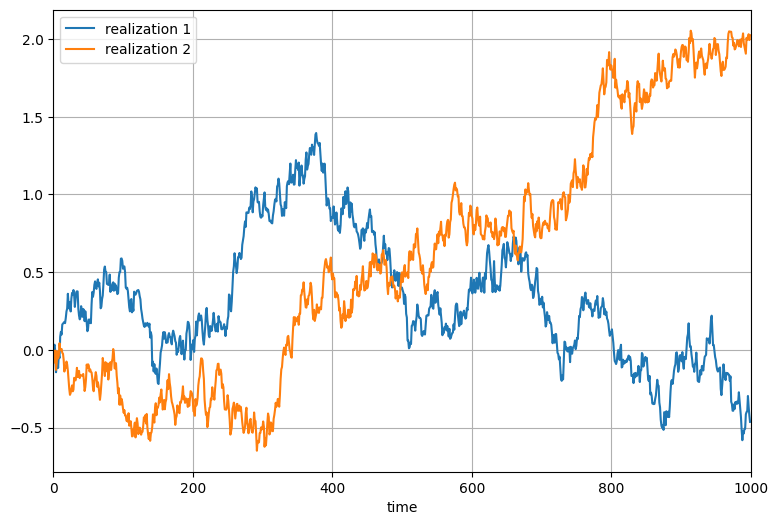
\includegraphics[width=0.5\linewidth]{addons/brownian_motion}
\end{center}
\label{fig:brownian_motion}
\end{figure}

\begin{question}
Using the Euler scheme simulate the 4-months (with daily steps) evolution of a Geometric Brownian Motion stochastic process with initial value $S_0=100$, $\mu=0.005$, and $\sigma=0.05$.
\end{question}

\cprotEnv\begin{question}
This \href{https://github.com/matteosan1/advanced_financial_modeling/raw/master/input_files}{file} contains a thousand 10-day realizations (with 0.1 day step) of historical price data of a single asset, assume that all the time series are different realizations of the same stochastic process.
\begin{itemize}
\item Make two figures: the first should contain one realization as a function of time, in the second plot the first 50 realizations together as a function of time (\emph{label the axes appropriately}).
\item In two separated plots report the mean and the variance of the stock prices as a function of time (\emph{label the axes appropriately}).
\item Perform the variable change $X_{n+1}=\log\left(\cfrac{S_{n+1}}{S_n}\right)$ on $S_{n+1} = S_ne^{(\mu-0.5\sigma^2)\Delta t + \sigma\sqrt{\Delta t}Z}$ to rewrite the model into a simpler form. 
	\begin{itemize}
	\item Is the resulting dynamics linear ? Prove it, or give a counterexample; 
	\item is the resulting system time-invariant ? Prove it, or give a counterexample.
	\end{itemize}
\item Apply again the same transformation $X_{n+1}=\log\left(\frac{S_{n+1}}{S_n}\right)$ to data this time. Plot both the mean and the variance of the transformed realizations as a function of time.
\end{itemize}

\noindent
\textbf{Hint:} the input file is a binary file that can be loaded back using \texttt{numpy} as follows (replace the URL from the link above):
\begin{ipython}
import numpy as np

path = np.DataSource("https://github.com/matteosan1/...../input_files")
S = np.load(path.open("stock_2023.npy", "rb"))
\end{ipython}
\end{question}

\begin{question}

The Heston model can be considered an extension of the Black and Scholes model where the volatility of the underlying asset is not constant, nor even deterministic, but follows a random process.

The basic Heston model assumes that $S_t$, the price of the asset, follows
\begin{equation}
dS_{t}=\mu S_{t}\,dt+{\sqrt {\nu _{t}}}S_{t}\,dW_{t}^{S}
\end{equation}
where the volatility 
\begin{equation}
{\displaystyle d\nu _{t}=\kappa (\theta -\nu _{t})\,dt+\xi {\sqrt {\nu _{t}}}\,dW_{t}^{\nu },}
\end{equation}
and 
\begin{equation}
W_{t}^{S},W_{t}^{\nu }
\end{equation} 
are Wiener processes with correlation $\rho$.

The model has five parameters:
\begin{itemize}
\item $\nu _0$, the initial variance;
\item $\theta$, the long variance of the price; as $t$ tends to infinity, the expected value of $\nu_t$ tends to $\theta$;
\item $\rho$, the correlation of the two Wiener processes;
\item $\kappa$, the rate at which $\nu_t$ reverts to $\theta$;
\item $\xi$, the volatility of the volatility, which determines the variance of $\nu_t$.
\end{itemize}

Using the Euler scheme simulate a possible realization for $S$ and $\sigma$ using the parameters: $\nu _0=0.02760$, $\kappa=1.2$, $\theta=0.066$, $\xi=0.593$, $\rho=0.659$.
\end{question}

\section{Floating Rate Notes}
Floating rate bond or note (FRN) usually refers to an instrument whose coupon is based on a short term rate (3-month T-bill, 6-month LIBOR). Variable coupon rates are fixed in advance at reset dates, which are 3- or 6-month (interest payment period) earlier.

In this example we use an annual payment frequency but the extension to the quarterly or semi-annual frequency is straightforward.

Floating rate bond price with (\emph{unit notional amount}), $n$ maturity, annual frequency ($\tau=1$), and the first coupon rate predetermined at previous reset date ($C_{reset}$) is as follows.

\begin{equation}
\begin{aligned}
\textbf{FRN} & = D_{0,1}C_{reset} + \sum_{i=1}^nD_{0,i}f_{i,i+1} + D_{0,n}= \\
& = D_{0,1}C_{reset} + D_{0,2}f_{1,2} + \ldots + D_{0,n-1}f_{n-2,n-1}+ D_{0,n}(1+f_{n-1,n}) = \\
& = D_{0,1}C_{reset} + D_{0,2}\left(\frac{D_{0,1}}{D_{0,2}}-1\right) + \ldots \\
&\quad\ldots + D_{0,n-1}\left(\frac{D_{0,n-2}}{D_{0,n-1}}-1\right) + D_{0,n}\left(\frac{D_{0,n-1}}{D_{0,n}}-1\right) + D_{0,n} = \\
& = D_{0,1}C_{reset} + (D_{0,1} - D_{0,2}) + (D_{0,2} - D_{0,3}) + \ldots \\
&\quad\ldots + (D_{0,n-2} - D_{0,n-1}) + (D_{0,n-1} - D_{0,n}) + D_{0,n} = \boxed{D_{0,1} (1 +C_{reset})}
\end{aligned}
\end{equation}
where $f(t_1,t_2)$ denotes the forward rate between $t_1$ and $t_2$.

If the remaining maturity of the above \textbf{FRN} for example was 4.25 year, its price will be
\begin{equation}
\textbf{FRN} = D_{0,\frac{1}{4}}(1+C_{reset})
\end{equation}

If the remaining maturity of the above \textbf{FRN} was $(4 + \epsilon)$ year, in this case, the price would be

\begin{equation}
\begin{aligned}
\textbf{FRN} &= D_{0,1}f_{0,1}+ D_{0,2}f_{1,2} + \ldots + D_{0,n-1}f_{n-2,n-1} + D_{0,n}(1+f_{n-1,n}) = \\
& = D_{0,1}\left(\frac{D_{0,0}}{D_{0,1}}-1\right) + D_{0,2}\left(\frac{D_{0,1}}{D_{0,2}}-1\right) + \ldots \\
&\quad\ldots + D_{0,n-1}\left(\frac{D_{0,n-2}}{D_{0,n-1}}-1\right) + D_{0,n}\left(\frac{D_{0,n-1}}{D_{0,n}}-1\right) + D_{0,n} = \\
&= (D_{0,0}-D_{0,1})+(D_{0,1}-D_{0,2}) + \ldots \\
&\quad\ldots + (D_{0,n-2}-D_{0,n-1})+(D_{0,n-1}-D_{0,n})+D_{0,n} = 1
\end{aligned}
\end{equation}

The price of FRN has a range from \emph{par} to \emph{par} + full coupon. It is par right before the reset date and is $C$ right after the reset date (and is linear when pricing date is between two reset dates).

\begin{question}
Draw a plot showing the characteristic sawtooth behaviour of a floating rate note. The relevant insterest rates can be taken from \href{https://raw.githubusercontent.com/matteosan1/advanced\_financial\_modeling/master/input_files/libor.csv}{libor.csv}
\end{question}

\section{Importance Sampling}
Assume we want to calculate the expectation $\mathbb{E}[f(X)]$
\begin{equation}
\mathbb{E}[f(X)] = \int_{-\infty}^\infty f(x)p(x)dx
\end{equation}
where $p(x)$ is the probability density function associated to the random variable $X$.

We can approximate this expectation using numerical approximation, i.e. Monte Carlo simulation, by sampling $n$ random values from the distribution $p$ and then calculating the sample mean as:
\begin{equation}
\bar{f}(x) = \frac{1}{n}\sum_i f(x_i)
\end{equation}

The idea behind \textbf{importance sampling} is to use a simple re-formulation trick and write the expectation in a slightly different form
\begin{equation}
\mathbb{E}[f(X)] = \int_{-\infty}^\infty f(x)\frac{p(x)}{q(x)}q(x)dx
\end{equation}
giving the expectation of $f(x)\frac{p(x)}{q(x)}$ over the distribution $q$. And with that, allowing us to calculate the sample mean by sampling from $q$:
\begin{equation}
\bar{f}(x) = \frac{1}{n}\sum_i f(x_i)\frac{p(x)}{q(x)}
\label{eq:reformulated_expectation}
\end{equation}

\subsection{Variance Reduction}
From probability theory we know that the variance of the standard Monte Carlo estimator is given by:
\begin{equation}
\cfrac{1}{n}\cdot\text{Var}[f(x)] = \cfrac{1}{n}\cdot\mathbb{E}[(f(X)-\mathbb{E}[f(X)])^2]
\end{equation}

Hence the variance for the re-formulated importance sampling estimator in Eq.\ref{eq:reformulated_expectation} is:
\begin{equation}
\cfrac{1}{n}\cdot\text{Var}\left[\cfrac{p(x)}{q(x)}f(x)\right]
\end{equation}

This give us a hint on how to find a way to reduce the variance. And indeed it is relatively easy to see that this variance could be reduced to 0 by choosing $q$ as:
\begin{equation}
\begin{aligned}
q(x)&=\cfrac{f(X)p(x)}{\mathbb{E}[f(X)]} \implies \cfrac{1}{n}\cdot\text{Var}[\mathbb{E}[f(X)]] = \cfrac{1}{n}\cdot\mathbb{E}[(\mathbb{E}[f(X)]-\mathbb{E}[\mathbb{E}[f(X)]])^2]=\\
&=\cfrac{1}{n}\cdot\mathbb{E}[(\mathbb{E}[f(X)]-\mathbb{E}[f(X)])^2] = 0
\end{aligned}
\end{equation}

Naturally, we don’t know $\mathbb{E}[f(X)]$, as the reason we are doing this sampling after all is to find the expectation of $f$.
However, we can think of the denominator of the previous expression as some normalisation constant, and consider to construct $q$ such that it has \textbf{high} density wherever $f(x)p(x)$ is \textbf{high}.

\subsection{Practical Example}
For the sake of demonstration, we choose $f=\mathcal{N}(5, 1)$, and the probability distribution $p=\mathcal{N}(9,2)$ which do not overlap too well, see Fig.\ref{fig:f_and_p}.
\begin{figure}[htbp]
\begin{center}
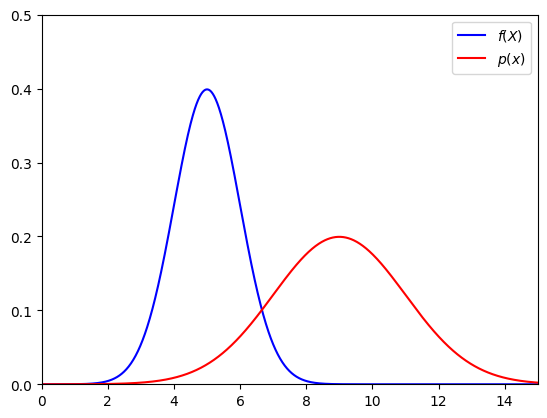
\includegraphics[width=0.5\linewidth]{addons/f_and_p}
\end{center}
\label{fig:f_and_p}
\end{figure}

To approximate numerically the expectation, as stated above, we would now sample values $x_i$ from the distribution $p$, and compute the mean of $f(x_i)$.

Intuitively one can see why sampling from this distribution is a bad idea: for most values sampled from $p$, $f$ will be close to 0, but for a few sampled values $f$ will be very large, thus we obtain a large variance.

\begin{figure}[htbp]
\begin{center}
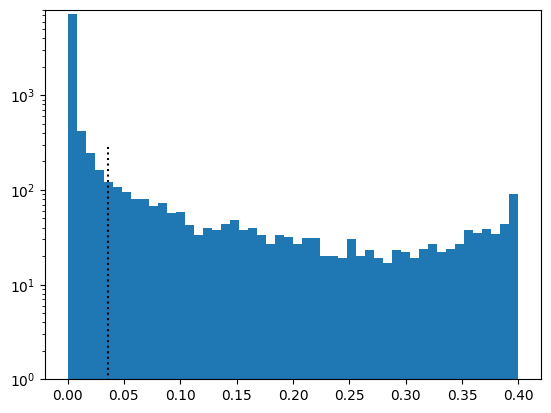
\includegraphics[width=0.5\linewidth]{addons/bad_sampling}
\end{center}
\label{fig:bad_sampling}
\end{figure}

Looking at Fig.|\ref{fig:bad_sampling} it is apparent how the vast majority of samples piles up at 0 (notice the logarithmic scale of the plot). 
Therefore, as outlined above, to make the sampling more efficient, we can try a new distribution $q = \mathcal{N}(5.8, 1)$, which satisfies the criterion that its pdf is high in regions where $f(x)p(x)$ is high, see Fig|\ref{fig:fp_and_q}.

\begin{figure}[htbp]
\begin{center}
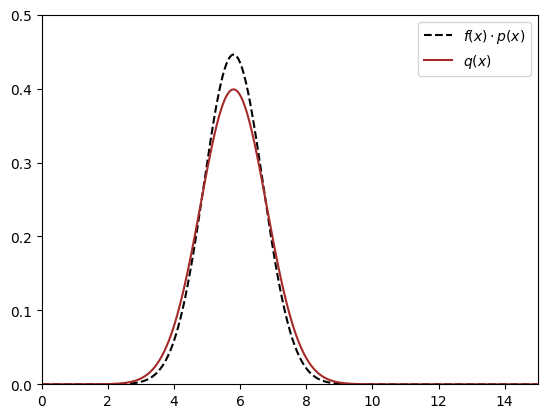
\includegraphics[width=0.4\linewidth]{addons/fp_and_q}
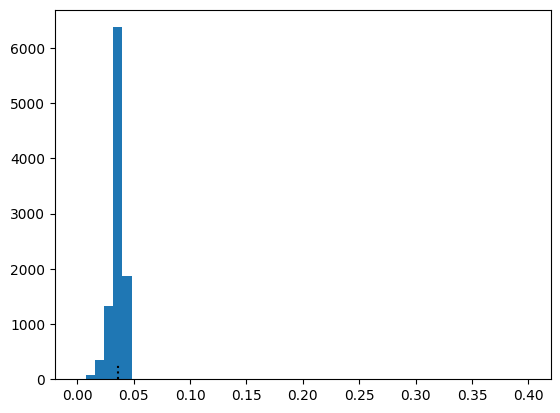
\includegraphics[width=0.4\linewidth]{addons/good_sampling}
\end{center}
\label{fig:fp_and_q}
\end{figure}

The resulting sampling is much better since the values are now clustered around 0.03. Comparing the estimates of the expectation in the two cases shows that the value is essentially the same, but the variance almost a factor 200 lower when using the importance sampling.
\begin{ioutput}
Numerical Simulation: mean 0.03611, variance 0.00759
Importance Sampling: mean 0.03603, variance 0.00003
\end{ioutput}
Note that in general it’s not trivial at all to find $q$, and certainly there are much more difficult real-word scenarios. For this example I actually plotted $p(x)f(x)$ and then picked a $q$ which resembled it best.

\begin{question}
Implement the importance sampling example outlined above, trying to reproduce the results quoted in the text.
\end{question}
\begin{question}
Estimate how unlucky is a 25 standard deviation return
\begin{equation*}
\theta := P(X\geq 25) = \mathbb{E}[\mathbbm{1}_{X\geq 25}]  \quad\text{where } X\sim \mathcal{N}(0, 1)
\end{equation*}
\end{question}
\begin{question}
Consider a one year ($T=1$) call option with $S_0=100$ , $K=170$,  $\sigma=0.2$, and $r=0.06$. The option is far out of the money, assuming we need to estimate its valye using Monte Carlo simulation, improve the efficiency of the calculation with importance sampling.

\noindent
Interesting reference \emph{Variance Reduction Techniques of Importance Sampling Monte Carlo Methods for Pricing Options}, 
Journal of Mathematical Finance, 2013, 3, 431-436.
\end{question}

\section{Reverse Floater}

* For instance, in September 2009, the short-term interest rate, the 3-month EURIBOR, **was at 0.5%**, and the forward curve was rising rather steeply, i.e. the implied forward 3-month EURIBOR in 3 years **was at 3.3%**. 
* The 3-year interest rate for a fixed-coupon bond **was at 3.5%** at the time. 
* It was possible to construct a 3-year reverse floater bond paying:

$$ 6\% - 2 \cdot \text{3M-EURIBOR}$$

(the coupon payments usually occur on a quarterly basis). 
* Should the 3-Month EURIBOR not move during the first year, the coupon would amount to $6\% - 2 \cdot 0.5\% = 5\%$. 
* Compared to a floating rate bond, the outperformance would be 4.5% for that period. 
%* After 3 years, the invested nominal is redeemed along with the last coupon.

Vega 

$$V_{\text{cap}}=F\Phi(d_1) - K\Phi(d_2)$$

$$\nu = \frac{\partial V_{\text{cap}}}{\partial\sigma} =
F\phi(d_1)$$

\begin{figure}[htbp]
	\begin{center}
		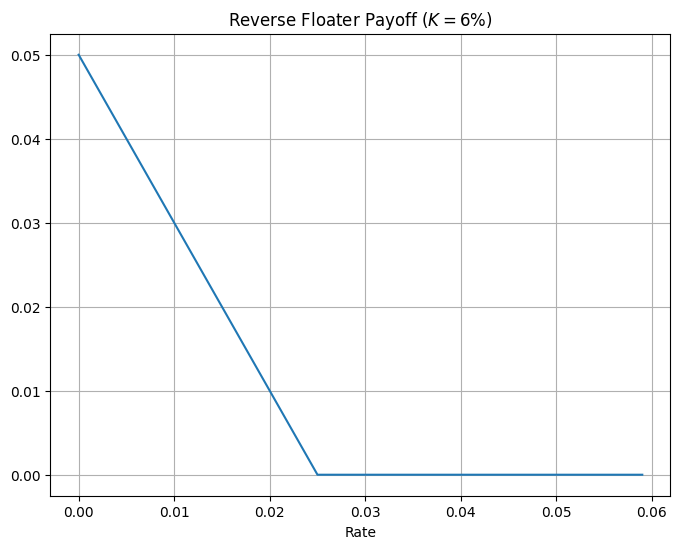
\includegraphics[width=0.5\linewidth]{addons/reverse_floater_payoff}
	\end{center}
	\label{fig:revere_floater_payoff}
\end{figure}

\begin{figure}[htbp]
	\begin{center}
		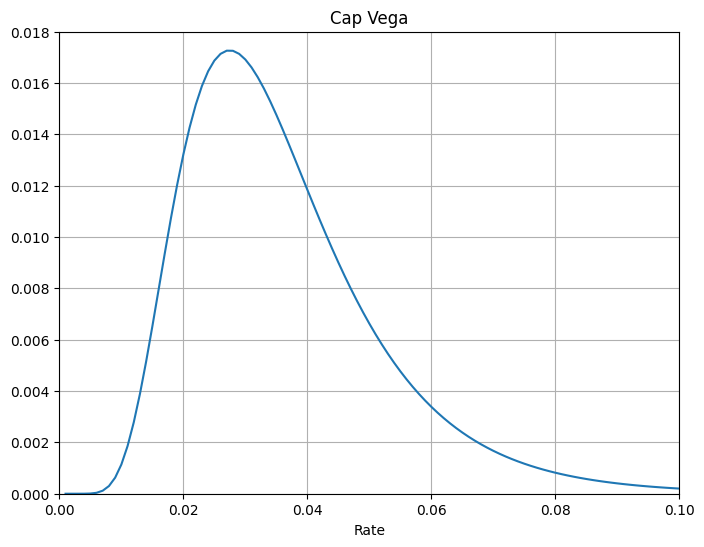
\includegraphics[width=0.5\linewidth]{addons/cap_vega}
	\end{center}
	\label{fig:cap_vega}
\end{figure}

\section{Interest Rate Swap as FRAs}

\section{Girsanov Theorem}
Let’s start with a standard Brownian motion $W_t^{\mathbb{P}} = \mathcal{N}_{\mathbb{P}(0,t)$ under a probability measure $\mathbb{P}$, and adapted to a filtration $\mathcal{F}_t$. These are 30 simulated evolution paths of $W_t^{\mathbb{P}}$, showing no drift, as expected:
	
\begin{figure}[htbp]
	\begin{center}
		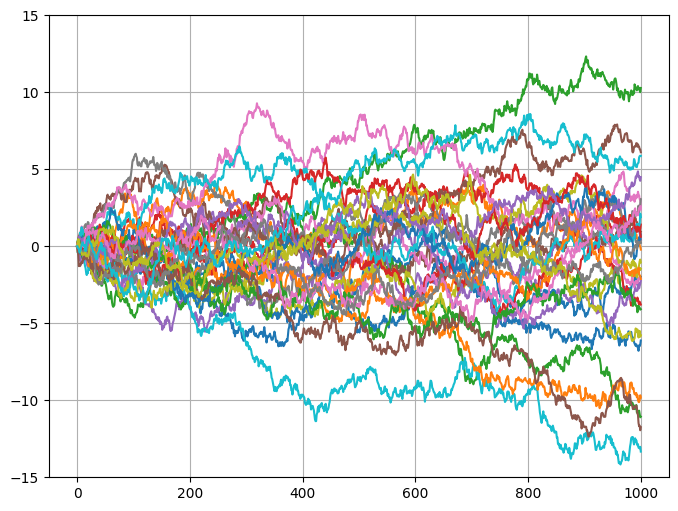
\includegraphics[width=0.5\linewidth]{addons/brownian_motion_nodrift}
	\end{center}
	\label{fig:brownian_motion_nodrift}
\end{figure}

For exemplification, let us now construct a "drifty" process $Y_t=\mu t+\sigma W_t^{\mathbb{P}}\in \mathcal_{\mathbb{P}}(\mu t, \sigma^2 t)$, that is, with drift $\mu$ and diffusion $\sigma$; in other words, $\mathbb{E}^{\mathbb{P}[Y_t]=\mu t$ and $\text{Var}^{\mathbb{P}}[Y_t]=\mathbb{E}^{\mathbb{P}[Y^2_t]-\mathbb{E}^{\mathbb{P}[Y_t]^2=\sigma^2 t$.

Incidentally, note the terminology: the drift is not an expectation, but rather the rate of change in expectation, and the diffusion is not a standard deviation, but rather the square root of the rate of 
change in variance. These are 30 simulated paths for the evolution of $Y_t$, for $\mu = 0.8$ and $\sigma =1.25$ (the drift is visually apparent):
\begin{figure}[htbp]
\begin{center}
	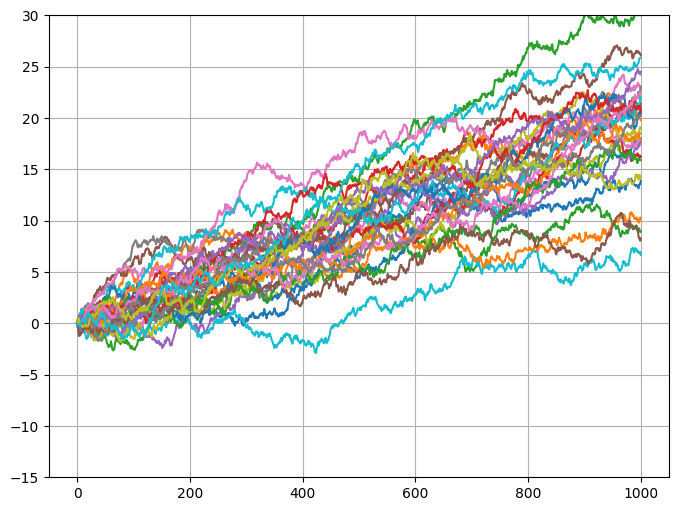
\includegraphics[width=0.5\linewidth]{addons/brownian_motion_drift}
\end{center}
\label{fig:brownian_motion_drift}
\end{figure}

We aim at applying a change of measure from $\mathbb{P}$ into a new probability $\mathbb{Q}$, such that $Y_t$ becomes driftless (a martingale) under $\mathbb{Q}: \mathbb{E}^{\mathbb{Q}}[Y_t]=0$, yet with the same diffusion as under $\mathbb{P}$: $\text{Var}^{\mathbb{Q}}[Y_t]=\sigma^2 t$

Consider the new process $U_t=\frac{1}{\sigma}Y_t\in\mathcal{N}_{\mathbb{P}}\left(\frac{\mu}{\sigma}t,t\right)$. In what follows, we will remove the drift of $U_t$, then reconstruct $Y_t$. For that, we follow Girsanov’s statement backwards: we aim at expressing $U_t$ as a standard Brownian motion under a probability $\mathbb{Q}$, that is, by Girsanov’s formula, we want to express $U_t$ in the following form:
\begin{equation}
	U_t = W_t^{\mathbb{P}} - [W_t^{\mathbb{P}}, M_t^{\mathbb{P}}]
\end{equation}
and now, we solve this equation for $M_t^{\mathbb{P}}$.
We ask ourselves the question: what process $M_t^{\mathbb{P}}$ satisfies ? ,
t
P P PP
t t tt
U
tW W W M µ
σ
+=−

? One can easily see that
the process P P M W t t
µ
σ = − verifies the expression , , PP P P P WM W W W t tt t t t
µµ µ
σσ σ = − =− =− ,
hence , P PP U W WM tt tt = − . Therefore P P M W t t
µ
σ = − is our solution. We use P Mt to define the
change of measure: Zt M ( ) = ε ( t )

\begin{figure}[htbp]
	\begin{center}
		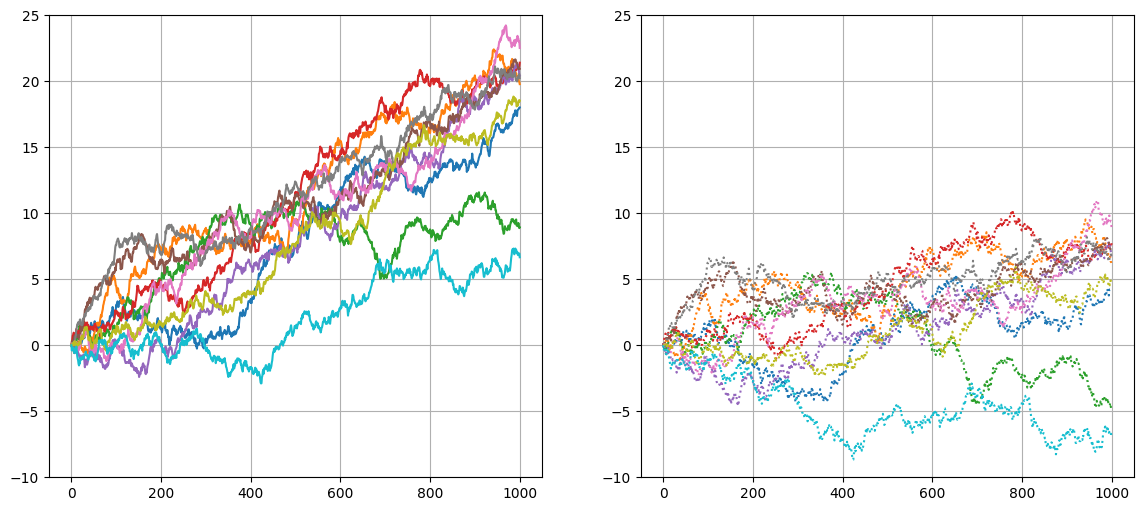
\includegraphics[width=0.5\linewidth]{addons/brownian_motion_girsanov}
	\end{center}
	\label{fig:brownian_motion_girsanov}
\end{figure}


\end{document}
